\section{Theoretical Framework}\label{sec:theoryFrames}
This section provides a brief explanation of the key concepts used in this research. Figure \ref{fig:conceptMap} summarizes the various concepts and their relationships.

\begin{figure*}[ht]
  \centering
  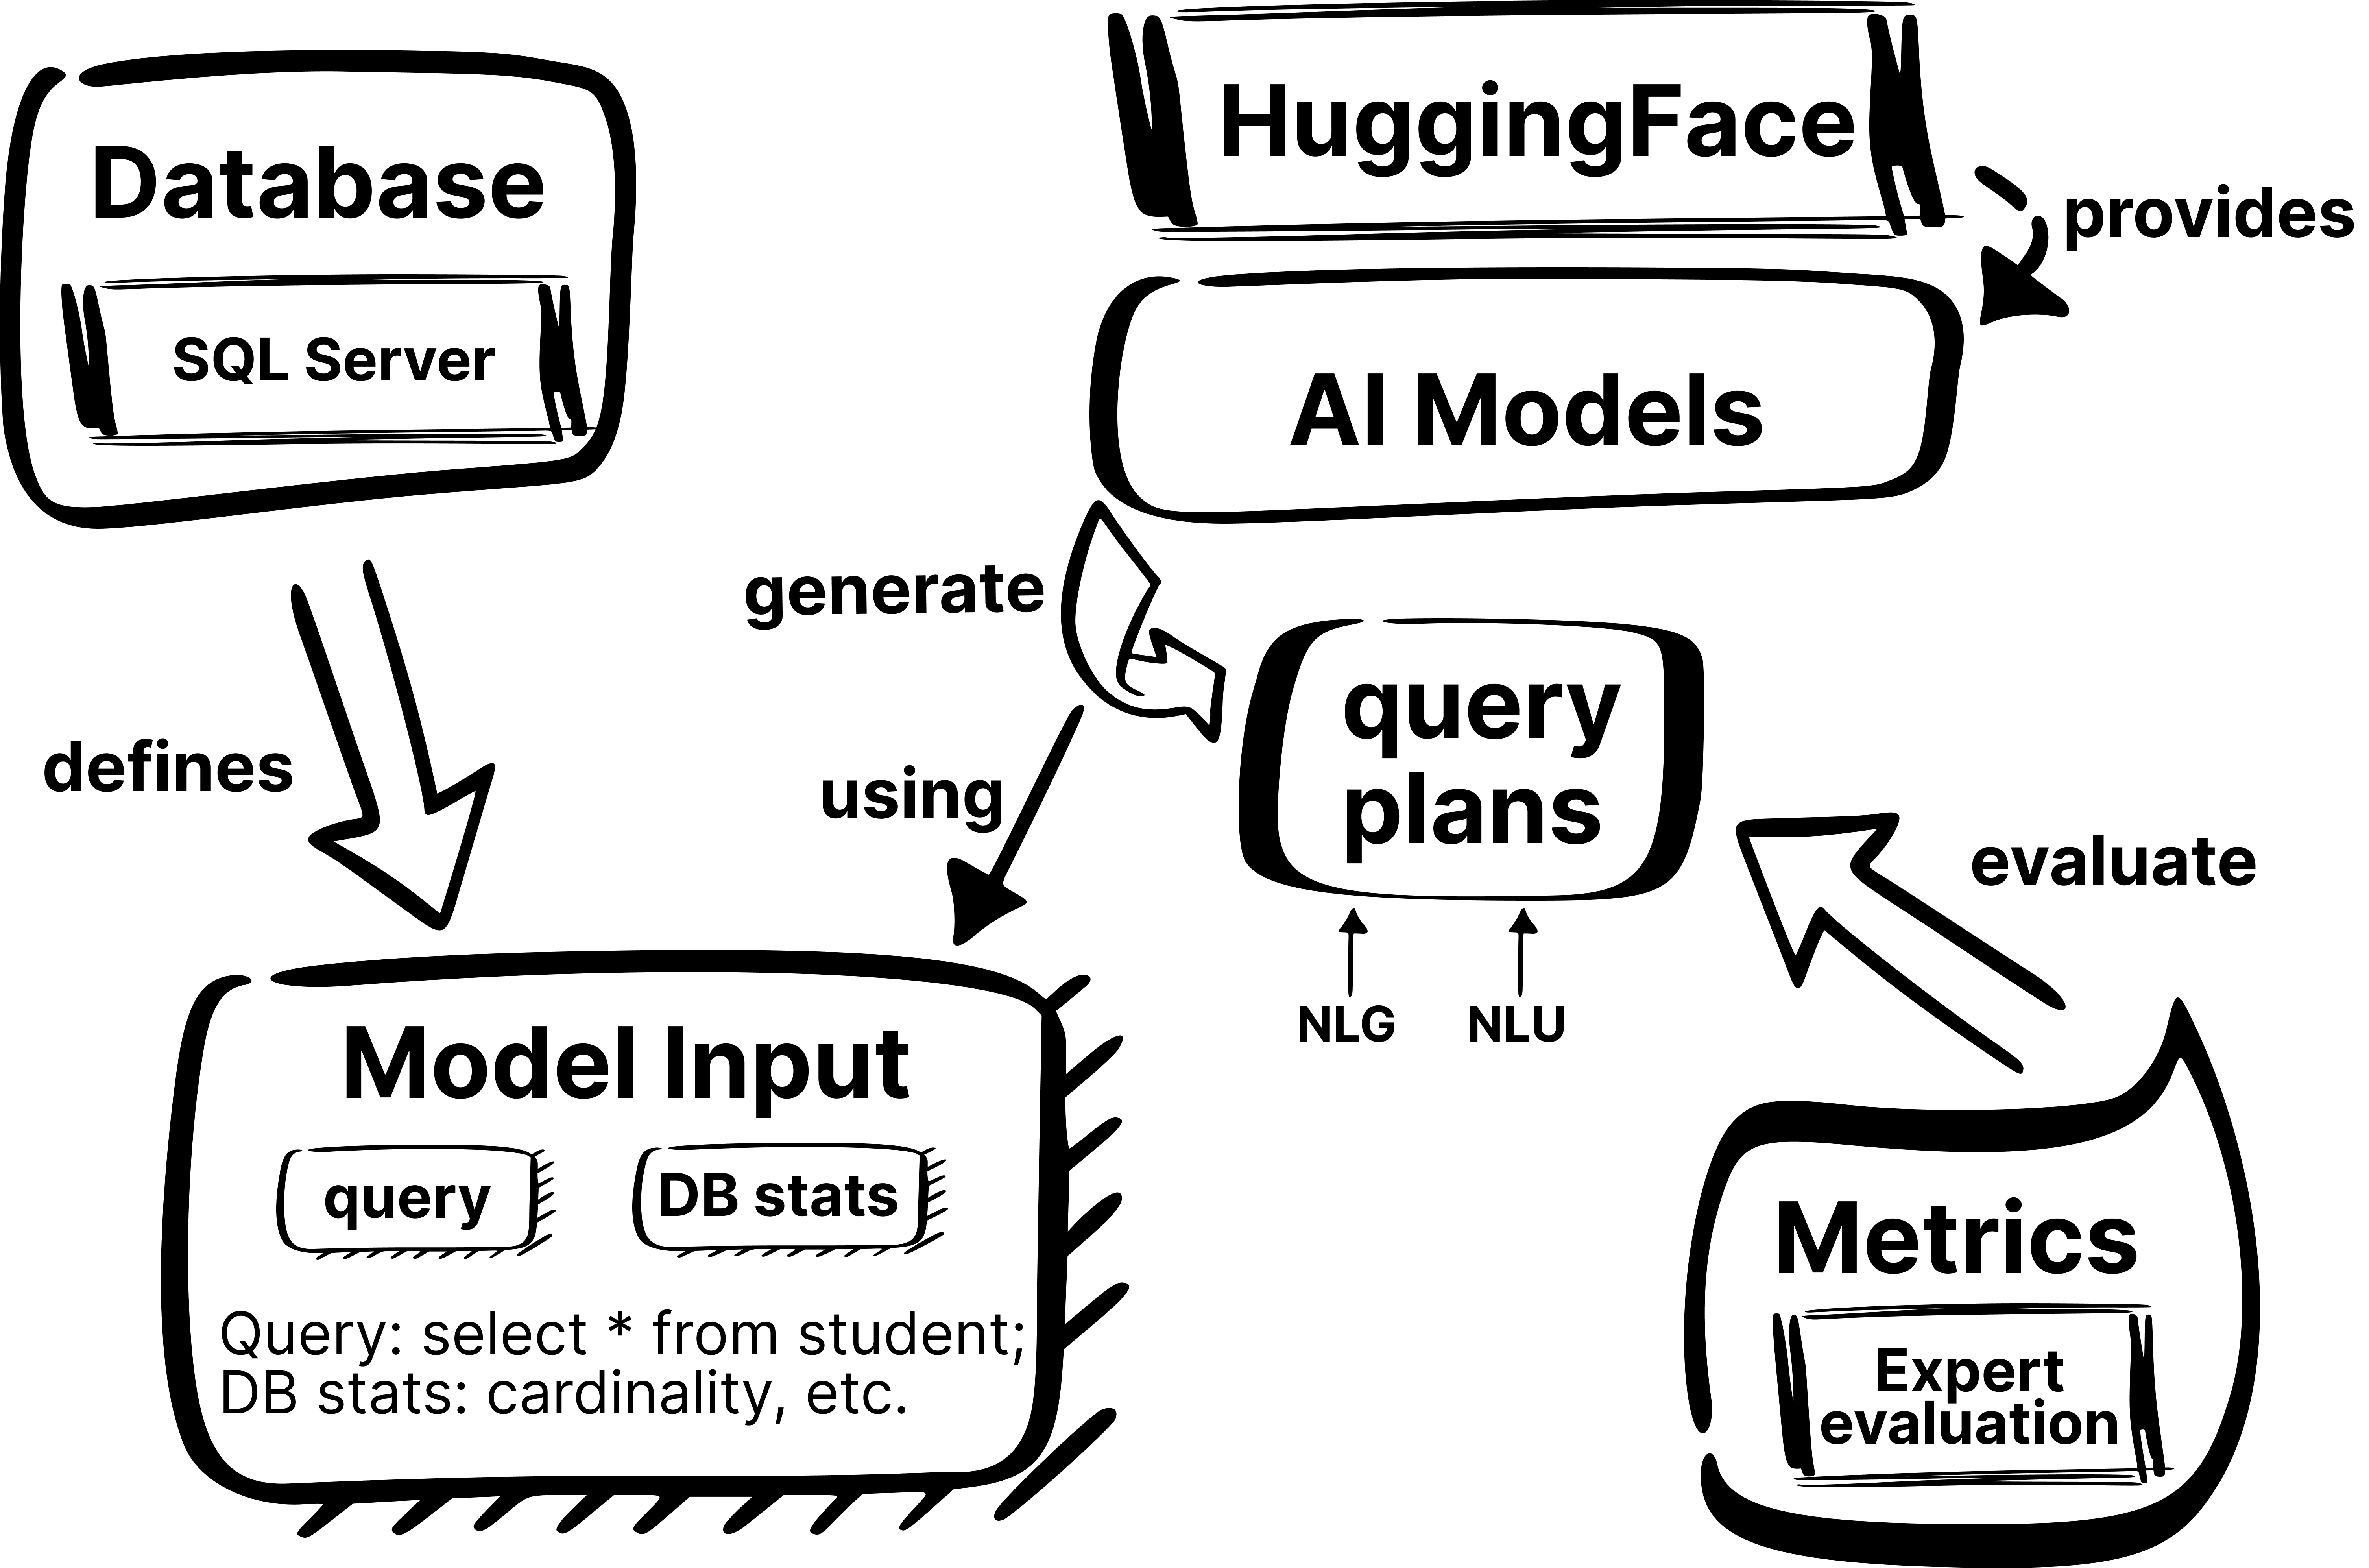
\includegraphics[width=\textwidth]{figures/llamaInferenceConceptMap.png}
  \caption{Concept map}
  \label{fig:conceptMap}
\end{figure*}


\subsection{Natural Language Processing}
QAG belongs to a broad field of problems involving machines and human language. These problems can be divided into several categories.

K. R. Chowdhary defines one category, natural language processing (NLP), as ``a collection of computational techniques for automatic analysis and
representation of human languages, motivated by theory'' \cite{chowdhary2020}. NLP ranges from simpler functionality such as spell checking to more challenging problems like the retrieval of important information. Some NLP problems can be further categorized under natural language understanding (NLU). NLU is a more advanced form of NLP in which machines understand language using background information much like humans do. NLU requires semantic information, abstract concepts, and various modules.

Chowdhary separates natural language generation (NLG) from NLP, categorizing both as branches of computational linguistics. While NLP is focused on language analysis, NLG involves machines writing human language rather than just reading and understanding it.

While these categories have different goals, NLG is interconnected with NLP. To generate text, a machine must first achieve a level of NLU. Because QAG requires a machine to generate natural language to achieve the desired output, it is considered part of NLG.

\subsection{AI Models}
Stanford University's Human-Centered Artificial Intelligence (HAI) institute cites the original definition of artificial intelligence (AI), ``the science and engineering of making intelligent machines,'' coined by John McCarthy in 1955\footnote{\href{https://hai.stanford.edu/sites/default/files/2020-09/AI-Definitions-HAI.pdf}{hai.stanford.edu}}. This definition relies on the definition of intelligence, which the HAI defines as the ability to learn. Hence, it follows that \textit{artificial} intelligence is identified by a machine's ability to learn.

In \textit{Machine Learning: An Artificial Intelligence Approach} \cite{michalski2014}, Michalski et al. introduce the necessity of this type of learning by explaining that some tasks are simply too difficult to ``laboriously program'' into a computer. In other words, AI allows computers to perform tasks that humans perform but cannot fully articulate algorithmically. Rather than explicitly programming billions of decisions with conditional statements (\textit{if} this \textit{then} do that), machine learning allows a computer to ``learn by example'' and program these ``decisions'' automatically.

\subsection{Machine Learning}
Machine learning (ML) is a broad term for the process by which a computer constructs an AI model to perform a task. Arthur Samuel, who coined the term \cite{zhou2021}, defined ``machine learning'' as the ``field of study that gives computers the ability to learn without being explicitly programmed.'' Machine learning can take many different forms such as logistic regression, Naive Bayes, or clustering. In this thesis, we focus on deep learning.

\subsection{Deep Learning}
Michael Nielsen provides an excellent introduction to deep learning and neural networks in \textit{Neural Networks and Deep Learning} \cite{nielsen2015}. Deep learning is a subset of machine learning used to train neural networks. The fundamental unit of such a network is often called a node, neuron, or perceptron (see Figure \ref{fig:perceptron}).
\begin{figure}[ht]
  \centering
  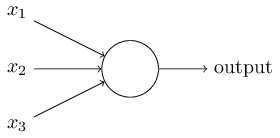
\includegraphics[width=0.5\textwidth]{figures/perceptron.png}
  \caption{A perceptron with three inputs $x_1$, $x_2$, and $x_3$ \cite{nielsen2015}}
  \label{fig:perceptron}
\end{figure}

An artificial neuron receives input, performs a mathematical (usually linear) transformation, and then returns some output, usually 0, 1, or some rational number in between. By combining many of these neurons in sequence, output to input, and in parallel, computer scientists construct neural networks (see Figure \ref{fig:perceptrons}).
\begin{figure}[ht]
  \centering
  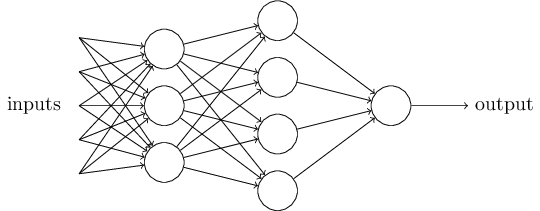
\includegraphics[width=0.7\textwidth]{figures/perceptrons.png}
  \caption{Connecting many perceptrons forms an artificial neural network \cite{nielsen2015}}
  \label{fig:perceptrons}
\end{figure}

The importance, or weight, of the connection between two perceptrons is the ``trainable'' part of the network. Deep learning uses backpropagation to adjust these connections by constantly taking partial derivatives between a provided example and the current state of each neuron. The neuron weights must be repeatedly tuned until the model can perform well with problems it has never seen before. Thus, to train a neural network using deep learning, we must possess many examples to present to the learning model. These examples are referred to as data.

\subsection{Data}
For a model to learn based on empirical evidence, it must be shown many examples representative of the target task. The success of this learning process relies on the format and quality of these examples. For this thesis, we plan to utilize two separate but similar datasets.

\subsection{Transformers}
Most QG systems before the 2010s were rule-based, systematically transforming a context from a declarative sentence to a question. The introduction of transformers revolutionized much NLG research including the field of question generation \cite{vaswani2017}. Because many more thorough explanations can be found online and in published research, we will only briefly explain transformers at a high level here. As the title of Vaswani et al.'s ``Attention is All You Need'' paper suggests, rather than using long short-term memory (LSTM), transformers leverage attention mechanisms and to allow a model to selectively retain pieces of important information from past input and output sequences. This provides the model with a selective but theoretically infinite memory. Self-attention allows words near each other to adjust each other's meanings. Moreover, unlike Recurrent Neural Networks (RNNs) which generate words in sequence by feeding output back into the model, transformers utilize positional encoding, allowing for faster inference and training. This architecture not only performs well in NLG tasks, but is also parallelizable, making transformer training on vast datasets much easier.

\subsection{Python and Libraries}
Due to the various state-of-the-art algorithms and resources included in LLM fine-tuning, research works commonly use Python for configuring their training experiments \cite{serban2016, kumar2021, ushio2022, goyal2023, ushio2023, hwang2023}. Python simplifies the implementation of these algorithms and the access to these resources through its vast amount of useful AI and data management libraries. For AI tasks, we plan to utilize a family of libraries released by HuggingFace\footnote{\url{https://huggingface.co/}} centered around the transformers library \cite{wolf2020}. To clean and format data we will use the Python libraries \lstinline{pandas} and \lstinline{numpy}.
